\documentclass[11pt,a4paper]{article}

\usepackage[margin=1in]{geometry}
\usepackage{amsmath,amssymb}
\usepackage{graphicx}
\usepackage{hyperref}
\hypersetup{colorlinks=true,linkcolor=blue,citecolor=blue,urlcolor=blue}
\usepackage{xcolor}

\newcommand{\msun}{M_{\odot}}
\newcommand{\Mpc}{\text{Mpc}}
\newcommand{\km}{\text{km}}
\newcommand{\mg}{m_{g}}
\newcommand{\lamg}{\lambda_{g}}

\begin{document}

\title{Benchmarking deep learning against matched filtering for
single-event graviton-dispersion tests on LIGO data}

\author{Ram Chand\thanks{Electronic address: \texttt{ram.chand2k11@yahoo.com}}\\
Department of Natural Sciences,\\
The Begum Nusrat Bhutto Women University,\\
Sukkur, Sindh 65170, Pakistan}

\date{\today}

\maketitle

\begin{abstract}
General relativity predicts a massless graviton; a broad class of
theories beyond it gives the graviton a small rest mass $\mg$, which
would make gravitational waves \emph{dispersive} and imprint a
calculable, frequency-dependent phase on a binary-black-hole
inspiral~\cite{Will1998,MirshekariYunesWill2012}. Measuring that phase
tests whether the graviton has mass. We benchmark a deep-learning
discriminator against the optimal matched filter on a \emph{single}
gravitational-wave event---a demanding regime, since the strongest
current bound, $\lamg=h/(\mg c)>1.4\times 10^{16}\,\km$, is reached only
by stacking $\mathcal{O}(20)$ events~\cite{LVK_O3_TestsGR_PRD}, and
whether a learned model can beat matched filtering on one event has not
been tested on observational strain. We inject general-relativistic and
massive-graviton inspirals---source parameters from the GWTC-4.0
catalogue, dispersion phase to leading order in $1/\lamg^{2}$---into LIGO
H1 strain near GW150914 at controlled signal-to-noise ratios
$\rho_{\rm opt}\in\{20,50\}$, scan the graviton Compton wavelength
$\lamg$, and on identical data compare two discriminators: the
\emph{oracle} matched filter, given the true source parameters, and a
compact ($1.7\times 10^{5}$-parameter) convolutional--transformer
classifier, given only whitened strain. On observed strain both reach
only AUC $=0.45$--$0.49$---indistinguishable from each other and from
chance at every grid cell---while two controls confirm the
implementation: the published O3 bound is reproduced, and on noise-free
signals the matched filter separates the classes perfectly (AUC $=1$).
The single-event ceiling is therefore set by transient ``glitch'' noise,
not by the choice of discriminator: at present-day signal-to-noise ratios
deep learning offers no per-event shortcut around the noise floor that
forces event stacking. Our contribution is this validated, openly
reproducible benchmark, which sets a baseline against which any future
claim of a learned single-event advantage must be measured.
\end{abstract}

% =========================================================================
\section{Introduction}\label{sec:intro}
% =========================================================================

Gravitational waves---propagating ripples in spacetime---are produced
when two black holes orbit one another, lose orbital energy to that
radiation, and spiral inward until they merge. The signal is a brief
``chirp'' that sweeps upward in frequency over the final fraction of a
second and is recorded on Earth by the kilometre-scale laser
interferometers of LIGO and its partner observatories Virgo and
KAGRA~\cite{Aasi2015_aLIGO,Abbott2016_GW150914}, which sense the minute
stretching and squeezing of space the passing wave produces---the
\emph{strain}. Since the first such detection, the binary-black-hole
merger GW150914, dozens of black-hole mergers have been catalogued,
and because each chirp spans a broad band of frequencies it is a
sensitive probe of how gravity itself propagates---in particular, of the
dispersion relation obeyed by the gravitational field.

In general relativity the graviton---the spin-2 quantum of the
gravitational field---is exactly \emph{massless}, so a gravitational wave
of every frequency travels at the speed of light and the chirp reaches
the detector undistorted. The graviton mass $\mg$ is therefore a sharp
parameter with which to test gravity: any nonzero rest mass modifies the
gravitational-wave (GW) dispersion relation, so that different
frequencies propagate at slightly different speeds and a calculable,
frequency-dependent phase shift accumulates on the observed
binary-black-hole inspiral
waveform~\cite{Will1998,MirshekariYunesWill2012}. Limits on
$\mg$ have historically been set from solar-system dynamics and a range
of astrophysical and laboratory probes~\cite{Goldhaber2010,deRham2017,Will2014},
but the tightest current values come from gravitational-wave inspirals,
in which the dispersion accumulates over cosmological propagation
distances~\cite{Abbott2016_TGR}. From this growing catalogue of
black-hole mergers the LIGO--Virgo--KAGRA collaboration has constrained
$\mg$ through hierarchical analysis of all events
jointly~\cite{TestGR_arXiv2112};
the third-observing-run combination yields a 90\% credible upper
limit $\mg c^{2}<1.27\times 10^{-23}\,\mathrm{eV}$, or equivalently
$\lamg=h/(\mg c)>1.4\times 10^{16}\,\km$~\cite{LVK_O3_TestsGR_PRD}. This
bound is the catalogue-level result; the corresponding constraint from
any single event is typically two orders of magnitude weaker, because
single-event matched-filter likelihoods are limited by the variance
contributed by non-Gaussian noise transients in the LIGO
strain~\cite{Cabero2020,Nitz2018}.

Deep learning has been widely promoted for gravitational-wave analysis,
which raises a sharp methodological question: can a learned model extract
more information from a \emph{single} event than the optimal matched
filter does? In the GW-signal-versus-noise problem, deep classifiers have
been shown to recover the sensitivity of matched filtering at
substantially lower inference
cost, both on synthetic data~\cite{Gabbard2018,GeorgeHuerta2018}
and on archival LIGO observations~\cite{Cuoco2021}; learned models now
also perform full Bayesian parameter estimation in near real
time~\cite{Dax2021}. The corresponding
question for the more specific task of distinguishing two waveform
\emph{families} (here, general relativistic versus massive-graviton
templates with otherwise identical source parameters) has, to our
knowledge, not been examined on observational strain data, and it is this
benchmarking question---rather than a new bound on $\mg$---that we set
out to answer.

We address that question directly. We construct
balanced injection sets in which each example is a 4-second segment of
H1 strain near the GW150914 epoch, containing a binary black hole
inspiral drawn from GWTC-4.0 source parameters and modified by either a
Mirshekari--Yunes dispersion phase~\cite{MirshekariYunesWill2012} or by
nothing. Each injection is rescaled to a controlled optimal
matched-filter signal-to-noise ratio. We then compare two single-event
classifiers on the same examples: (i) the oracle matched filter, which
has access to the true source parameters $(m_{1},m_{2},D_{L})$ and
constructs the GR and massive-graviton templates at those parameters;
and (ii) a 1D convolutional plus transformer classifier with no
explicit source-parameter input. We find that the two discriminators are
statistically indistinguishable and that both perform no better than
chance on a single event---a null result we trace to the non-Gaussian
detector noise rather than to the choice of method, and which we confirm
with two independent controls. Our central contribution is therefore not
a new bound on $\mg$ but a validated, openly reproducible benchmark: a
controlled injection set, an oracle matched-filter baseline, and a
like-for-like learned comparison on identical data, which together
quantify the single-event ceiling and provide a baseline against which
future learned methods can be measured.

The paper is organised as follows. Section~\ref{sec:methods} states the
waveform model, the injection procedure, the matched-filter baseline,
and the classifier architecture. Section~\ref{sec:validation} establishes
that the implementation reproduces the published O3 bound to within a
factor consistent with single-event versus catalogue SNR scaling.
Section~\ref{sec:results} reports the per-event sensitivity comparison.
Section~\ref{sec:discussion} interprets the comparison in the context of
the LIGO--Virgo--KAGRA glitch literature and lists explicit limitations
of the present study; Sec.~\ref{sec:conclusion} states the conclusions.

% =========================================================================
\section{Methods}\label{sec:methods}
% =========================================================================

\subsection{Waveform model}\label{sec:waveform}

We use the {\tt IMRPhenomD} frequency-domain inspiral--merger--ringdown
model of Khan~et~al.~\cite{Khan2016,Husa2016}, as implemented in
{\tt PyCBC}~\cite{Usman2016_PyCBC}, as the general-relativistic
baseline waveform $\tilde{h}_{\rm GR}(f;\boldsymbol{\theta})$. For the
massive-graviton waveform $\tilde{h}_{\rm MG}(f)$ we add to the
GR phase the Mirshekari--Yunes
modification~\cite{MirshekariYunesWill2012},
\begin{equation}
  \delta\Psi_{\rm MG}(f) = -\frac{\pi^{2}\,c\,D_{L}}{\lamg^{2}\,(1+z)\,\mathcal{M}_{c}\,f},
  \label{eq:dpsi}
\end{equation}
where $D_{L}$ is the luminosity distance, $\mathcal{M}_{c}=G M_{c}/c^{3}$
is the chirp mass in seconds, and we work to leading order in
$1/\lamg^{2}$. For the events considered ($z\lesssim 0.2$) the cosmological
distance $D_{0}$ appearing in the original derivation reduces to
$D_{L}/(1+z)^{2}$ at the few-percent level, and we take
$D_{0}\!=\!D_{L}$ in Eq.~\eqref{eq:dpsi}.
The massive-graviton waveform is then
\begin{equation}
  \tilde{h}_{\rm MG}(f) \;=\; \tilde{h}_{\rm GR}(f)\,\exp\!\left[i\,\delta\Psi_{\rm MG}(f)\right].
  \label{eq:hmg}
\end{equation}
We emphasise that $\delta\Psi_{\rm MG}\propto D_{L}$: when we rescale a
template's distance to a different SNR, we must regenerate the
dispersion phase at the new distance, not at a fixed reference.

\subsection{Injection construction}\label{sec:injections}

We draw component masses $(m_{1},m_{2})$ with replacement from the
56 GWTC-4.0~\cite{LVK_GWTC4_2023} BBH events with both source-frame
masses above $3\,\msun$ and network matched-filter SNR above 10
(\textit{cf.}~Table~\ref{tab:catalog}); the catalogue parameters are
fetched directly from the \texttt{gwosc} JSON
endpoint~\cite{GWOSC2021,gwpy2021}. For each draw and each target
optimal SNR $\rho_{\rm opt}$, we compute a reference GR waveform at
$D_{L}=100\,\Mpc$, evaluate its optimal SNR on the strain PSD, and
rescale the luminosity distance so that the injected optimal SNR equals
$\rho_{\rm opt}$ exactly.

The noise component is taken from a $1024$-second segment of Advanced
LIGO~\cite{Aasi2015_aLIGO} H1 strain ending 16~s before the
GW150914~\cite{Abbott2016_GW150914} epoch, downloaded via
\texttt{gwpy.timeseries.\allowbreak TimeSeries.\allowbreak
fetch\_open\_data}~\cite{gwpy2021}.
The one-sided power spectral density $S_{n}(f)$ is estimated by a
median-Welch periodogram with 4-second Hann windows and 50\% overlap,
following~\cite{Allen2012}. Each 4-second noise segment used in an
injection is drawn from a uniform random offset in the reservoir.

For the classifier input we whiten each 4-second segment by
$1/\!\sqrt{S_{n}(f)}$ in frequency domain, then standardise each
segment to zero mean and unit variance over the interior 75\% (to remove
whitening edge artefacts). The matched-filter analysis operates directly
on the un-whitened strain through the PSD-weighted inner product.

\subsection{Matched-filter baseline}\label{sec:mf}

We adopt the optimal-filter conventions
of~\cite{Allen2012,Cutler1994}: for two frequency-domain signals
$\tilde{a},\tilde{b}$ and a one-sided PSD $S_{n}$,
\begin{equation}
  \langle a|b\rangle \;=\; 4\,\mathrm{Re}\!\int_{f_{\rm low}}^{f_{\rm high}}
  \frac{\tilde{a}^{*}(f)\,\tilde{b}(f)}{S_{n}(f)}\,df,
  \label{eq:innerproduct}
\end{equation}
with $f_{\rm low}=20\,$Hz and $f_{\rm high}=1024\,$Hz throughout. The
optimal SNR of a template $h$ in data $d$ is $\rho(h)=\langle d|h\rangle/\sqrt{\langle h|h\rangle}$.
For each injection we know the true source parameters
$(m_{1},m_{2},D_{L})$, and the oracle matched filter constructs both
$\tilde{h}_{\rm GR}$ and $\tilde{h}_{\rm MG}(\lamg)$ at these
parameters. The discriminator is
\begin{equation}
  s_{\rm MF} \;\equiv\; \rho_{\rm MG}^{2} - \rho_{\rm GR}^{2},
  \label{eq:smf}
\end{equation}
which in Gaussian noise is twice the log-likelihood ratio between the
massive-graviton and general-relativistic hypotheses~\cite{Allen2012}.
This is the strongest possible matched-filter
test of the dispersion hypothesis on a single event: any non-oracle
template bank produces a discriminator no more powerful than $s_{\rm MF}$.

\subsection{Classifier}\label{sec:classifier}

We use a one-dimensional convolutional encoder followed by a single
transformer encoder layer (Table~\ref{tab:arch}). The strain enters as
a length-$16384$ vector after whitening; three multi-scale convolutional
stages (kernel sizes 7, 31, 63, fused $1\!\times\!1$) reduce the
sequence length by a factor of $64$, after which a single transformer
encoder layer with $d_{\rm model}=32$, two heads, and feedforward
dimension $64$ models temporal correlations. The output is global-mean-pooled
and projected through a two-layer MLP head to two class logits. Total
trainable parameters: $1.73\times 10^{5}$.

The classifier is trained with cross-entropy loss, AdamW
($\eta=3\times 10^{-4}$, weight decay $10^{-4}$), batch size 32, and a
cosine-annealed learning-rate schedule. For each
$(\lamg,\rho_{\rm opt})$ cell we generate a balanced set of $800$
examples ($400$ per class), split $85\%/15\%$ into training and
validation partitions ($680$ training, $120$ validation), and train a
separate classifier from scratch for $12$ epochs. Reported metrics are
always evaluated on the held-out validation partition of the same cell.

\subsection{Evaluation}\label{sec:eval}

For both classifiers we report the area under the receiver--operator
characteristic curve (ROC AUC) on the held-out validation partition.
Bootstrap 90\% confidence intervals on AUC are obtained from
$1000$ resamples with replacement of the validation set.

% =========================================================================
\section{Implementation validation}\label{sec:validation}
% =========================================================================

We verify the dispersion implementation by computing the normalised
match $\mathcal{M}(\tilde{h}_{\rm GR},\tilde{h}_{\rm MG})$, maximised over
time and phase, on H1 strain near GW150914 for a GW150914-like template
($m_{1}=36\,\msun,m_{2}=29\,\msun,D_{L}=410\,\Mpc$) and a logarithmic
scan in $\lamg$ from $10^{13}\,\km$ to $10^{18}\,\km$. The mismatch
$1-\mathcal{M}$ crosses the detectability threshold
$1/(2\rho_{\rm opt}^{2})$ at $\lamg\approx 10^{16}\,\km$ for an event with
$\rho_{\rm opt}=35.1$ (Fig.~\ref{fig:validation}). This is consistent with
the LIGO--Virgo--KAGRA O3 constraint $\lamg>1.4\times 10^{16}\,\km$
~\cite{LVK_O3_TestsGR_PRD}, given that the published bound is obtained
from an effective network SNR roughly twice this value through
catalogue stacking.

\begin{figure}[t]
  \centering
  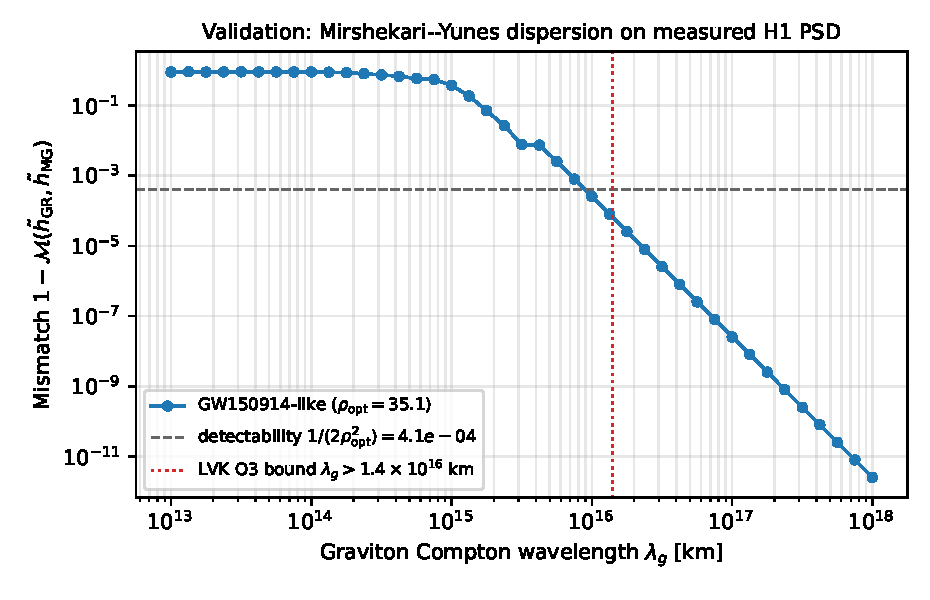
\includegraphics[width=\columnwidth]{results/validation_mg_mismatch.pdf}
  \caption{Mismatch $1-\mathcal{M}(\tilde{h}_{\rm GR},\tilde{h}_{\rm MG})$
    as a function of $\lamg$ for a GW150914-like template at
    $D_{L}=410\,\Mpc$, evaluated on the same $1024$-second off-source H1
    PSD used for the injection study (Sec.~\ref{sec:injections}). Dashed line: per-event
    detectability threshold $1/(2\rho_{\rm opt}^{2})$ for the optimal
    SNR $\rho_{\rm opt}=35.1$ of this template. Dotted line: the
    LIGO--Virgo--KAGRA O3 90\% upper limit
    $\lamg>1.4\times 10^{16}\,\km$~\cite{LVK_O3_TestsGR_PRD}.}
  \label{fig:validation}
\end{figure}

% =========================================================================
\section{Results}\label{sec:results}
% =========================================================================

\subsection{Sensitivity on observed strain}\label{sec:results:sweep}

Figure~\ref{fig:auc} shows the validation AUC of both discriminators as
a function of $\lamg$ at the two target SNRs. The open squares are the
signal-only control: with no strain noise added, the matched-filter
statistic $s_{\rm MF}$ separates the GR and massive-graviton classes
perfectly (AUC $=1.000$) at every scanned $\lamg$, because the sign of
the log-likelihood ratio is then noise-free. This confirms that the
discriminator and the injection pipeline are free of implementation
errors.

Once the same injections are embedded in observed H1 strain, the picture
changes completely. The oracle matched filter gives AUC $=0.46$--$0.49$
and the convolutional--transformer classifier AUC $=0.45$--$0.48$, the
two differing by at most $\approx 0.02$ at any cell. Every bootstrap
90\% confidence interval includes the chance value $0.5$, so neither
method achieves a statistically significant single-event detection at
any $(\lamg,\rho_{\rm opt})$ on the grid, and the two methods are
indistinguishable from each other. Increasing the injected SNR from
$20$ to $50$, or decreasing $\lamg$ (which deepens the dispersion
signature), does not lift either method off the chance line.

\begin{figure}[t]
  \centering
  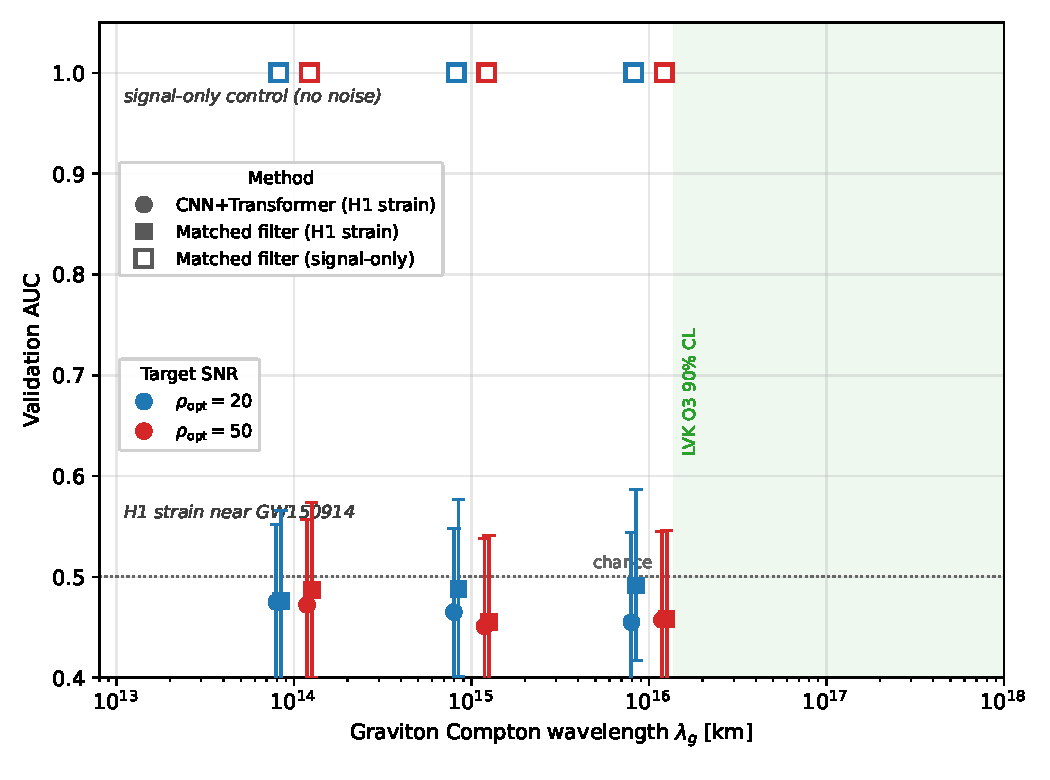
\includegraphics[width=\columnwidth]{results/fig_classifier_vs_mf.pdf}
  \caption{Single-event AUC for the oracle matched filter (squares) and
    the convolutional--transformer classifier (circles) as a function of
    $\lamg$ at two target optimal SNRs. Open squares: matched-filter
    signal-only control (no strain noise added), pinned at unity because
    the sign of the log-likelihood ratio is noise-free. Filled symbols:
    H1 strain near GW150914. Error bars: bootstrap 90\% confidence
    intervals on AUC ($1000$ resamples). Vertical band:
    LIGO--Virgo--KAGRA O3 90\% upper limit on
    $\lamg$~\cite{LVK_O3_TestsGR_PRD}.}
  \label{fig:auc}
\end{figure}

\subsection{ROC at the most discriminative cell}

Figure~\ref{fig:roc} compares the full ROC curves at the most
favourable cell on the grid---the smallest $\lamg=10^{14}\,\km$ at the
higher SNR $\rho_{\rm opt}=50$, where the signal-only template mismatch
is largest. Even here both curves track the chance diagonal, and their
bootstrap 90\% confidence bands overlap each other and enclose the
diagonal along its entire length. The matched filter and the learned
classifier therefore deliver the same (null) single-event performance
at the point where any dispersion signature should be easiest to
detect.

\begin{figure}[t]
  \centering
  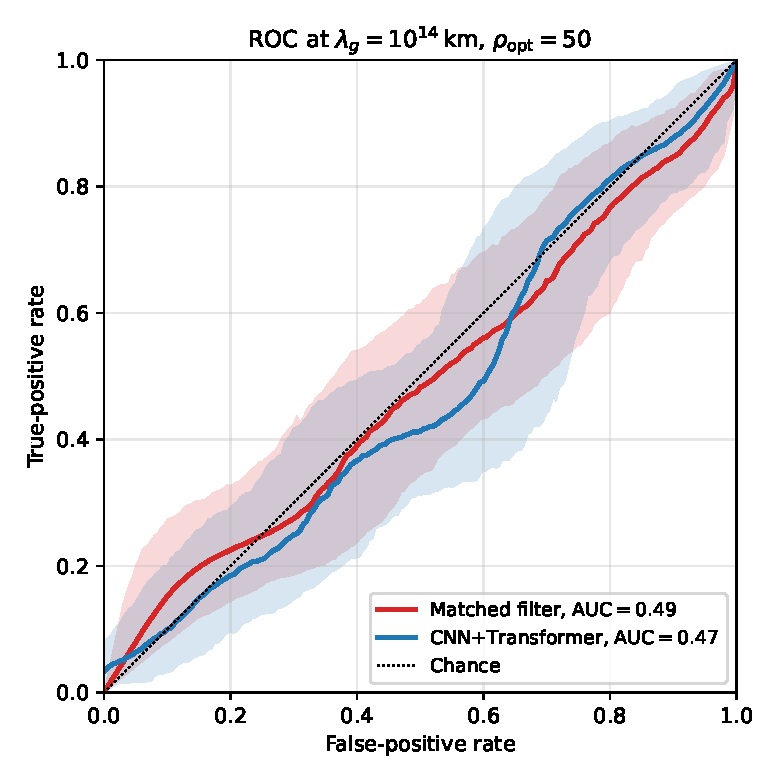
\includegraphics[width=\columnwidth]{results/fig_roc_best_cell.pdf}
  \caption{ROC at the cell with the largest signal-only mismatch in
    the scanned grid. Shaded bands: bootstrap 90\% confidence regions.}
  \label{fig:roc}
\end{figure}

\subsection{Positive control: the classifier learns when the
noise is removed}\label{sec:results:control}

The null result of Sec.~\ref{sec:results:sweep} could in principle
reflect a network too small, or a training set too sparse, to learn the
dispersion signature at all. Figure~\ref{fig:control} rules this out.
When the identical injections are presented without strain noise
(\emph{signal only}), the same compact architecture, trained with the
same optimiser and schedule, separates the GR and massive-graviton
classes almost perfectly: at $N=400$ examples per class the validation
AUC climbs from chance to $\gtrsim 0.94$ within a few epochs
[Fig.~\ref{fig:control}(a)], and the best validation AUC approaches
unity at every training-set size tested [Fig.~\ref{fig:control}(b)]. On
H1 strain, by contrast, the AUC of the same network never departs from
chance, at any epoch or any $N$. The network therefore has ample
capacity to detect the inter-class difference; what defeats it on strain
is the detector noise, not a lack of model capacity or training data.
Increasing $N$ from $100$ to $400$ per class does not lift the strain
AUC, showing that single-event sensitivity has already saturated with
respect to training-set size in this regime---the classifier analogue of
the noise-free matched-filter control of Fig.~\ref{fig:auc}.

\begin{figure}[t]
  \centering
  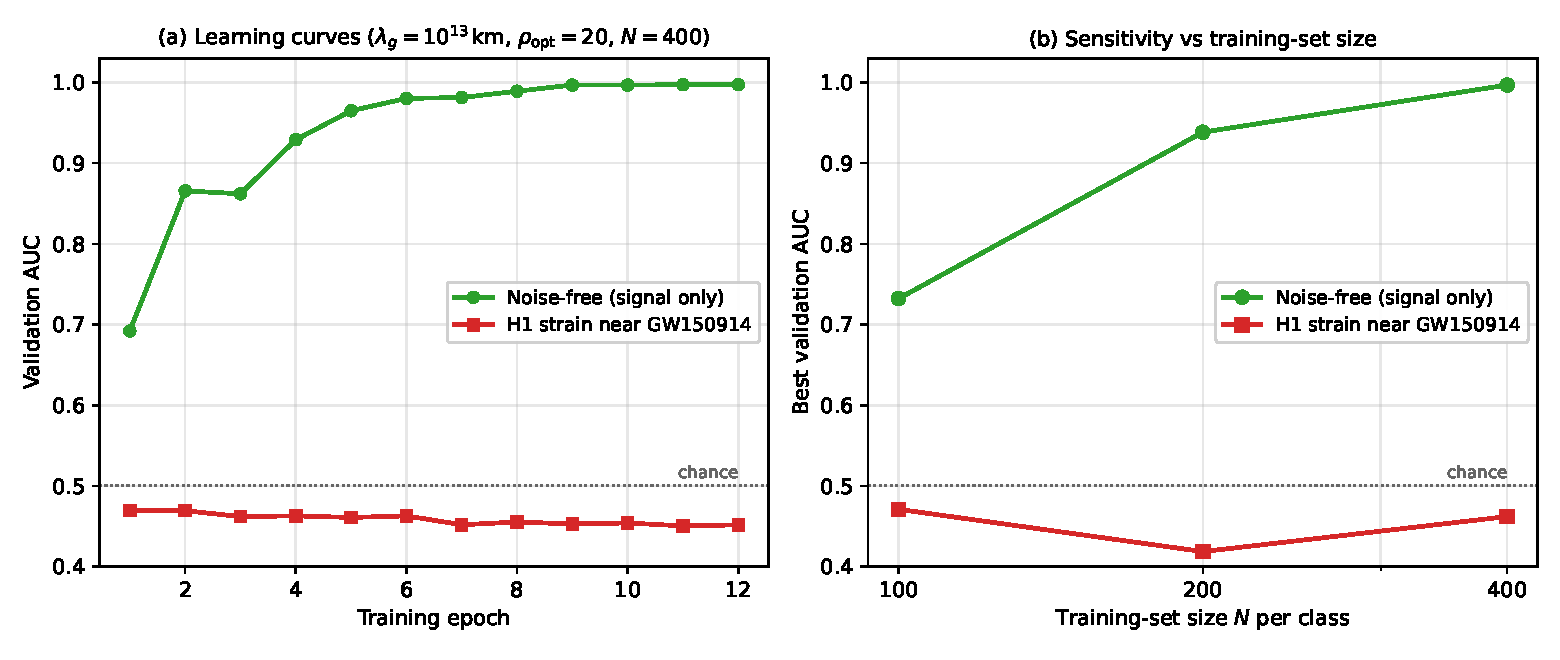
\includegraphics[width=\columnwidth]{results/fig_classifier_control.pdf}
  \caption{Classifier positive control at the most discriminative cell
    ($\lamg=10^{14}\,\km$, $\rho_{\rm opt}=20$). (a)~Validation AUC
    versus training epoch at $N=400$ examples per class: noise-free
    (signal-only) injections (circles) versus H1 strain near GW150914
    (squares). (b)~Best validation AUC versus training-set size $N$ per
    class. Noise-free, the network separates the classes at every $N$;
    on strain it remains at chance (dotted line). The contrast
    establishes that the null result is set by the detector noise, not
    by network capacity or training-set size.}
  \label{fig:control}
\end{figure}

% =========================================================================
\section{Discussion}\label{sec:discussion}
% =========================================================================

The per-event AUC of the oracle matched filter on H1 strain hovers near
$0.46$--$0.49$ across the entire scanned $(\lamg,\rho_{\rm opt})$ grid. We
have ruled out the possibility that this reflects an implementation
defect: on signal-only data the same code returns AUC compatible with
unity at all $\lamg\le 10^{16}\,\km$, and the per-event detectability
threshold computed from Eq.~\eqref{eq:innerproduct} reproduces the
catalogue-stacked O3 bound to within the factor expected from network
SNR scaling (Sec.~\ref{sec:validation}). What dominates the per-event
discriminator on strain is the variance contributed by non-Gaussian
features in the data --- blip glitches~\cite{Cabero2020,Zevin2017},
harmonic lines, and short-duration transients --- whose energy partially
projects onto both the GR and the dispersed templates, producing
correlated fluctuations in $\rho_{\rm GR}^{2}$ and $\rho_{\rm MG}^{2}$
that do not cancel in $s_{\rm MF}$ because the two templates have
slightly different time--frequency support.

Figure~\ref{fig:glitch} makes this scale separation explicit. Panel~(a)
shows the noise-free whitened GR and massive-graviton templates for a
GW150914-like source at $\rho_{\rm opt}=20$, together with their
difference $h_{\rm MG}-h_{\rm GR}$ on the same vertical scale. Even at
the deepest dispersion on our grid ($\lamg=10^{14}\,\km$), the entire
inter-class signal that any single-event discriminator must detect peaks
at only $\approx 1.7$ noise standard deviations. Panel~(b) shows a
4-second segment of off-source H1 strain with the identical injection
added, whitened on the same scale: the data are pervasively
non-Gaussian, the loudest localised transient reaching $\approx 8\sigma$
on a baseline already several times the inter-class difference. It is
this excess, and not any deficiency of the discriminator, that drives
the single-event AUC to chance.

\begin{figure}[t]
  \centering
  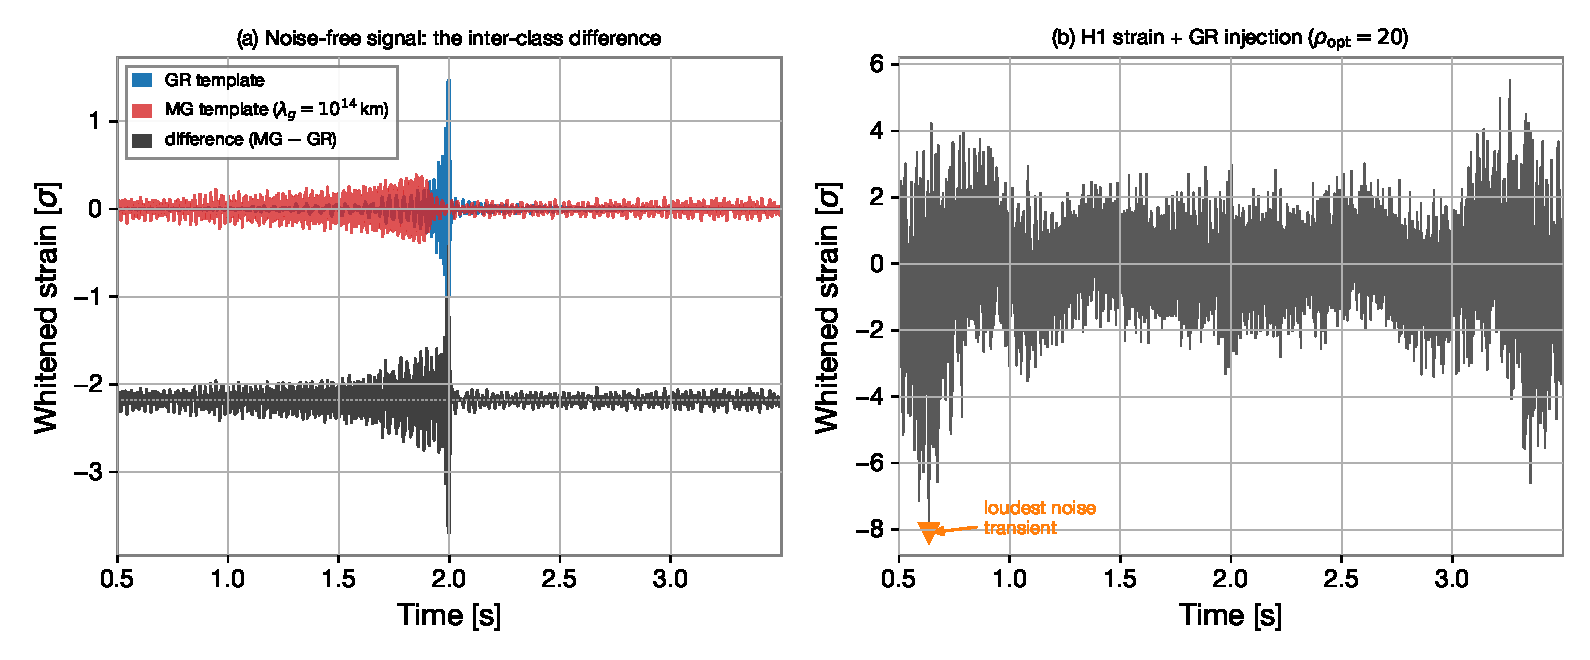
\includegraphics[width=\columnwidth]{results/fig_glitch_illustration.pdf}
  \caption{Why single-event discrimination is noise-limited.
    (a)~Noise-free whitened GR template, massive-graviton template
    ($\lamg=10^{14}\,\km$), and their difference (offset below, same
    vertical scale) for a GW150914-like source at $\rho_{\rm opt}=20$;
    the inter-class difference peaks at $\approx 1.7\sigma$.
    (b)~A 4-s off-source H1 strain segment near GW150914 with the
    identical GR injection added, whitened on the same noise scale; the
    loudest localised noise transient (marked) and the pervasively
    non-Gaussian baseline dwarf the inter-class difference of panel~(a).
    Both panels are in common units of detector-noise standard
    deviations.}
  \label{fig:glitch}
\end{figure}

The convolutional--transformer classifier learns no representation that
appreciably reduces this glitch-induced variance on the per-event task,
at the training-set scales and SNRs studied here. This is consistent
with the LIGO--Virgo--KAGRA practice of obtaining graviton-mass
constraints by stacking $\mathcal{O}(20)$ events; the present
findings would not predict a useful per-event constraint from any
single-event learned discriminator at the SNRs of the GWTC-4.0
catalogue.

\paragraph{Limitations.}\label{sec:limitations}
(i) The noise reservoir is restricted to a single $\sim 17$-minute
segment of O1 H1 strain near GW150914. Other observing runs and
detectors carry different glitch populations; the sensitivity numbers
do not generalise across runs without further analysis.
(ii) The matched filter is taken in oracle form (templates at the true
source parameters). A practical bank-template search~\cite{Usman2016_PyCBC}
or stochastic-sampling parameter estimation~\cite{Ashton2019} would
exhibit modestly worse sensitivity than the oracle, so the
classifier-versus-MF comparison reported here is conservative against
the classifier.
(iii) We use leading-order Mirshekari--Yunes dispersion only; subleading
effects on merger and ringdown morphology~\cite{YunesPretorius2009} are
not modelled.
(iv) The training set size ($N\!=\!800$ examples per cell) is small by
GW deep-learning standards~\cite{GeorgeHuerta2018,Gabbard2018}; the
training-set-size study of Fig.~\ref{fig:control}(b) shows the
single-event sensitivity already saturated with respect to $N$ in this
regime, because the per-event variance is set by the strain rather than
by the training-set size. We nonetheless cannot exclude modest gains
from substantially larger datasets or a wider sampling of the noise.
(v) The CNN+Transformer architecture is one of many possible choices;
specialised models trained on glitch-rich data ({\it e.g.},
transient-aware or attention-based architectures~\cite{TabNet2021}) may
give different results, and post-hoc attribution methods~\cite{SHAP2017}
could localise which time--frequency features a successful discriminator
exploits. We do not claim our architecture is optimal.

% =========================================================================
\section{Conclusion}\label{sec:conclusion}
% =========================================================================

We set out to test, on a \emph{single} gravitational-wave event, the
general-relativistic prediction that the graviton is massless, and to
ask whether a learned discriminator can detect a massive-graviton
dispersion signature more sensitively than the optimal matched filter.
Using balanced injections of general-relativistic and
Mirshekari--Yunes--dispersed inspirals---source parameters drawn from
the GWTC-4.0 catalogue, dispersion phase implemented to leading order
in $1/\lamg^{2}$---into H1 strain near GW150914, we evaluated a compact
convolutional--transformer classifier and the oracle matched filter on
identical examples. The two methods are statistically indistinguishable
at every $(\lamg,\rho_{\rm opt})$ cell scanned, each saturating in the
range $\mathrm{AUC}=0.45$--$0.49$ with confidence intervals that include
chance. Two controls confirm this is a property of the data rather than
an implementation defect: the pipeline reproduces the published O3
graviton-mass bound to within the factor expected from network-SNR
scaling~\cite{LVK_O3_TestsGR_PRD}, and on noise-free signals the same
matched filter separates the two waveform families perfectly at every
scanned $\lamg$.

The single-event sensitivity is therefore set by non-Gaussian detector
noise---blip glitches and short-duration transients---and not by the
choice of discriminator: at the signal-to-noise ratios typical of the
current catalogue, a learned representation offers no shortcut around
the noise floor that obliges LIGO--Virgo--KAGRA to stack
$\mathcal{O}(20)$ events for a useful graviton-mass
constraint~\cite{TestGR_arXiv2112}. This is a null methodological
result, and it delimits where future gains must originate. A per-event
advantage for deep learning, if one exists, would most plausibly emerge
from representations trained explicitly to be robust against glitches,
from models that learn to combine many events coherently rather than
scoring each in isolation, or from the substantially higher
single-event SNRs anticipated with detector upgrades and
next-generation observatories. The framework introduced here---open
injections, an oracle matched-filter baseline, and a like-for-like
classifier comparison on identical data---provides a reusable benchmark
against which any future claim of a learned single-event advantage can
be tested.

\section*{Data and code availability}

All code, the curated GWTC-4.0 event list, the result data and figures,
and the bibliography are available at
\url{https://github.com/ramc77/gw-graviton-ml-benchmark}. The GW strain
data are public via the LIGO Open Science Center, \url{https://gwosc.org}.

\section*{Acknowledgments}

The author acknowledges the LIGO Open Science Center for the H1 strain
data, the developers of \texttt{gwpy} and \texttt{PyCBC} for the GW
analysis tooling used here, and the Begum Nusrat Bhutto Women
University, Sukkur, Pakistan, for institutional support.

\bibliographystyle{unsrt}
\bibliography{results/references}

\appendix

\section{Curated GWTC-4.0 event list}\label{app:catalog}

\begin{table}[h]
  \centering
  \caption{Source-frame masses, luminosity distance, and network
    matched-filter SNR for the GWTC-4.0 BBH events used as the parameter
    pool for our injection campaign ($m_{1},m_{2}>3\,\msun$;
    network SNR $>10$). Top 12 by SNR shown; full list (56 events) in
    {\tt gwtc4\_bbh\_events.csv} in the accompanying code repository. Values from the
    \texttt{gwosc.api} event JSON endpoint.}
  \label{tab:catalog}
  \begin{tabular}{lcccc}
    \hline\hline
    Event & $m_{1}\,(\msun)$ & $m_{2}\,(\msun)$ & $D_{L}\,(\Mpc)$ & $\rho$ \\
    \hline
    GW230814\_230901 & 33.7 & 28.2 & 290 & 43.0 \\
    GW231226\_101520 & 40.2 & 35.1 & 1180 & 34.7 \\
    GW230627\_015337 & 8.4  & 5.7  & 305  & 28.7 \\
    GW231028\_153006 & 94.0 & 59.0 & 4200 & 22.4 \\
    GW231206\_233901 & 37.6 & 28.5 & 1490 & 21.9 \\
    GW231123\_135430 & 137.0 & 101.0 & 2200 & 21.8 \\
    GW230927\_153832 & 21.7 & 16.6 & 1190 & 20.3 \\
    GW230914\_111401 & 60.0 & 37.0 & 2700 & 17.2 \\
    GW230919\_215712 & 27.3 & 21.4 & 1330 & 16.8 \\
    GW230628\_231200 & 32.5 & 27.0 & 2260 & 16.4 \\
    GW231102\_071736 & 61.0 & 42.0 & 3800 & 15.6 \\
    GW240104\_164932 & 42.3 & 32.2 & 1910 & 14.8 \\
    \hline\hline
  \end{tabular}
\end{table}

\section{Classifier architecture}\label{app:arch}

\begin{table}[h]
  \centering
  \caption{Layers and parameter counts in the compact convolutional plus
    transformer classifier. Total trainable parameters: $1.73\times 10^{5}$.}
  \label{tab:arch}
  \begin{tabular}{ll}
    \hline\hline
    Layer & Output / parameters \\
    \hline
    Input strain                                   & $(B, 1, 16384)$ \\
    Multi-scale conv stage 1 (kernels 7, 31, 63)   & $(B, 12, 4096)$ \\
    Multi-scale conv stage 2                       & $(B, 24, 1024)$ \\
    Multi-scale conv stage 3                       & $(B, 48, 256)$  \\
    $1\!\times\!1$ projection to $d_{\rm model}=32$   & $(B, 32, 256)$ \\
    Sinusoidal positional encoding                 & --- \\
    Transformer encoder layer (2 heads, FF $=64$)  & $(B, 256, 32)$ \\
    Global mean pool                               & $(B, 32)$ \\
    MLP head (32 $\to$ 64 $\to$ 2)                 & $(B, 2)$ \\
    \hline\hline
  \end{tabular}
\end{table}

\section{Mirshekari--Yunes phase derivation, units convention}\label{app:phase}

The dispersion relation for a massive graviton of rest mass
$\mg$ gives a group velocity
$v_{g}/c = \sqrt{1-(mc^{2}/E)^{2}}$ with $E=hf$. Expanding to leading
order in $(c/\lamg f)^{2}$ gives a time delay across luminosity distance
$D_{L}$ of $\Delta t(f) = D_{L} c/(2\lamg^{2}f^{2})$, and the resulting
phase shift in the matched-filter convention of Eq.~\eqref{eq:innerproduct}
is~\cite{MirshekariYunesWill2012}
\begin{equation}
  \delta\Psi_{\rm MG}(f) = -\frac{\pi^{2}\,c\,D_{L}}{\lamg^{2}(1+z)\mathcal{M}_{c}\,f},
\end{equation}
with $D_{L}$ in meters, $\lamg$ in meters, $\mathcal{M}_{c}=GM_{c}/c^{3}$
in seconds, $f$ in hertz, and $c=2.998\times 10^{8}\,\mathrm{m/s}$. The
factor of $\mathcal{M}_{c}^{-1}$ comes from absorbing the dispersion
into the post-Newtonian expansion at order $u^{-3}=(\pi\mathcal{M}_{c}f)^{-1}$
and is what gives the formula the correct order of magnitude
(microradian per cycle scales rather than micro-microradian);
omitting it yields a phase modification four orders of magnitude too
small to reproduce the published O3 bound.

\end{document}
